\documentclass{beamer}
\usepackage{amsthm}
\usepackage{amssymb}
\usepackage{amsmath}
\usepackage{amsfonts}
\usepackage{graphicx}
\usepackage{tikz}
\usetheme{Rochester}
\usecolortheme{seahorse}
\usefonttheme{structuresmallcapsserif}
\setbeamertemplate{caption}[numbered]
\setbeamertemplate{footline}[frame number]
\usepackage{subfigure}
\newcommand{\myitem}{\item[$-$]}

\title{Efficient segmentation algorithms for shark fin identification}
\subtitle{Honours project proposal by Lize Cilli\'{e}}
\author{Project advisors: Prof. B.M.
Herbst and Dr. S.J. van der Walt}
\date{August 1, 2013}
\institute{Division of Applied Mathematics, Stellenbosch University}

\begin{document}
\maketitle


\begin{frame}
\frametitle{Motivation and problem statement}
\begin{itemize}

\item Motivation behind the project.
\begin{itemize}
\myitem Sharks have an unique dorsal fin structure.
\myitem The value of analysing shark fins.
\myitem PhD student in Marine Biology at Stellenbosch University, Ms. Sara
Andreotti and her work.
\myitem Databases of shark fin images.
\myitem Goal: group photos of a certain individual together.
\myitem Focus on distribution and movements of sharks rather than developing new software.
\myitem Advantage for marine scientists.
\end{itemize}
\pause
\item Methodology.
\begin{itemize}
 \myitem We will investigate different methods for classifying the foreground and
background and segmenting the foreground successfully for matching. 
\end{itemize}
\pause
\item Examples of shark fins.
\end{itemize}
\end{frame}


\begin{frame}
\frametitle{Examples of shark fin images showing the unique part of the dorsal fin}
\begin{figure}
\centering
\mbox{\subfigure[Shark fin 1]{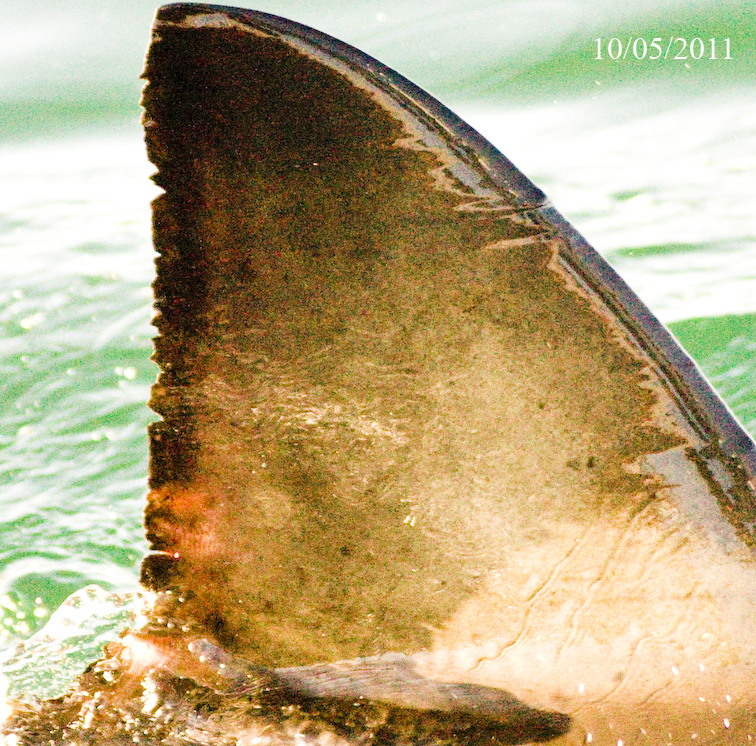
\includegraphics[width=1in]{haai1.jpg}} \quad
\subfigure[Shark fin 2]{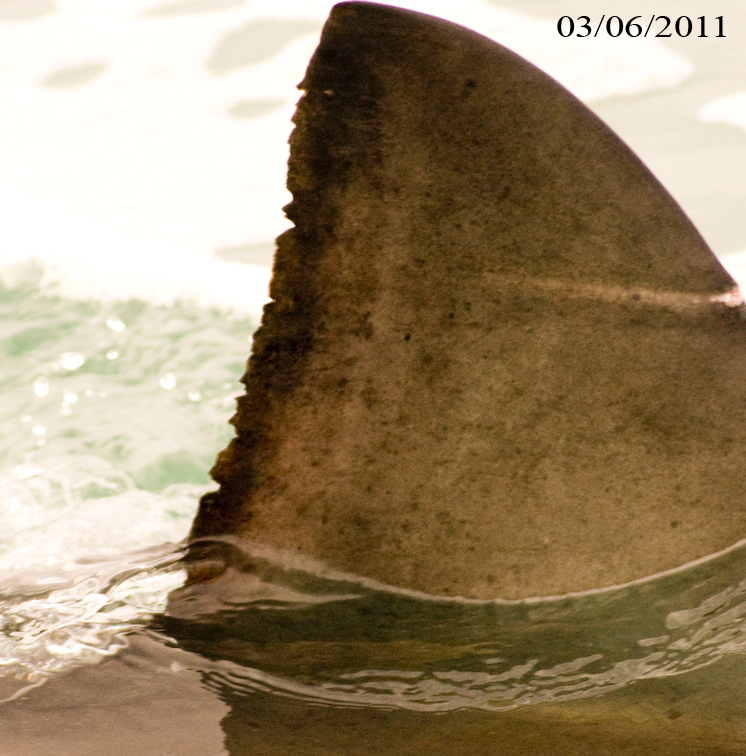
\includegraphics[width=1in]{haai2.jpg}}}
\end{figure}
\begin{figure}
\centering
\mbox{\subfigure[Shark fin 3]{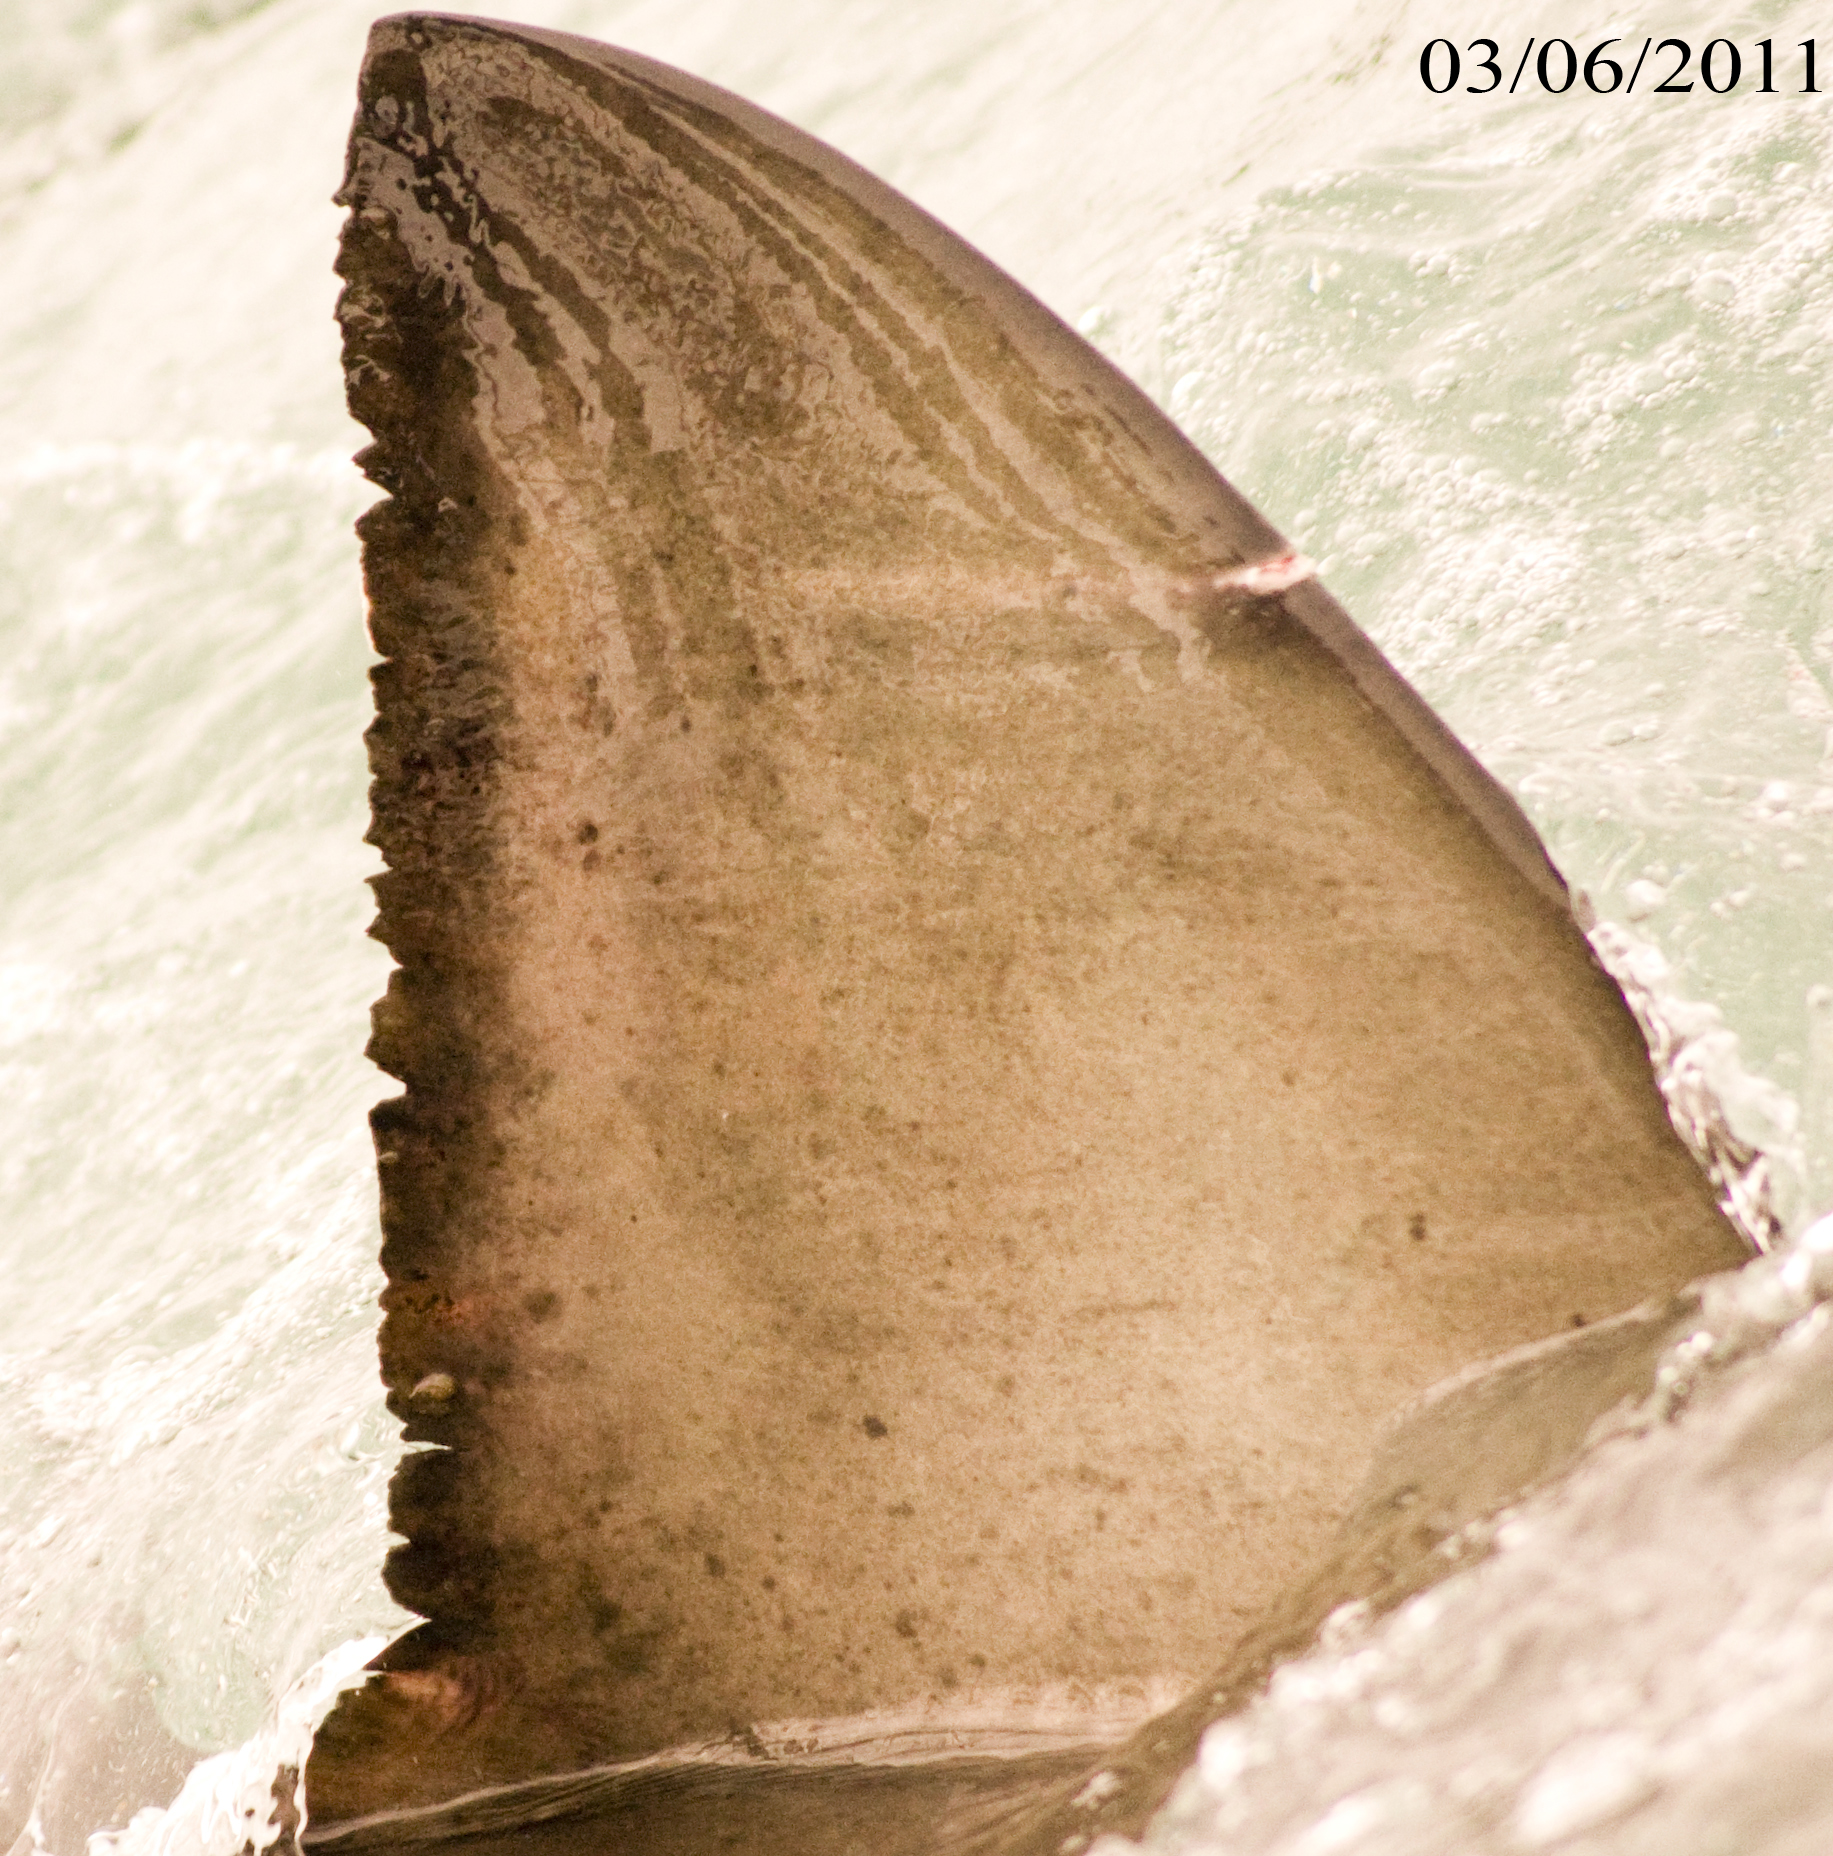
\includegraphics[width=1in]{haai3.jpg}} \quad
\subfigure[Shark fin 4]{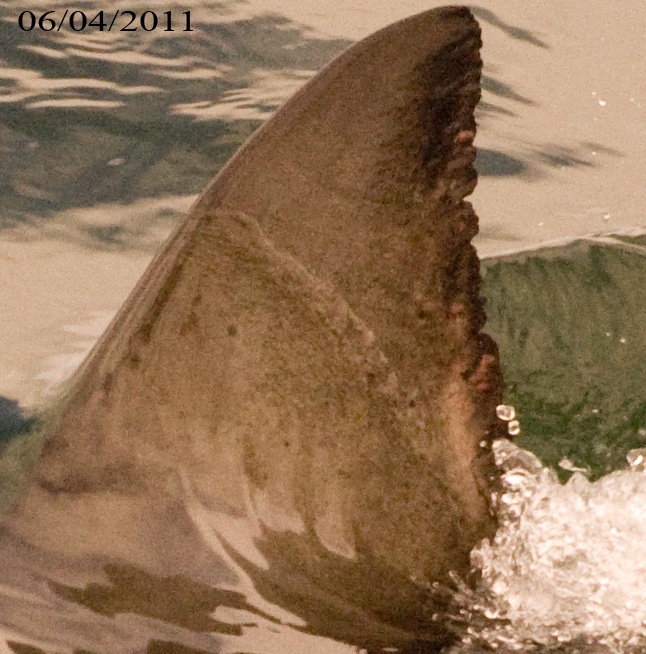
\includegraphics[width=1in]{haai4.jpg}}}
\end{figure}
\end{frame}


\begin{frame}
\frametitle{Background -- Image segmentation}
\begin{itemize}
\item Basic principle of segmentation algorithms.
\begin{itemize}
\myitem Partitioning a digital image into multiple segments to locate an object or
boundaries in the image.
\end{itemize}
\pause
\item Applications.
\begin{itemize}
\myitem Medical imaging to locate tumours.
\begin{figure}
 \centering
 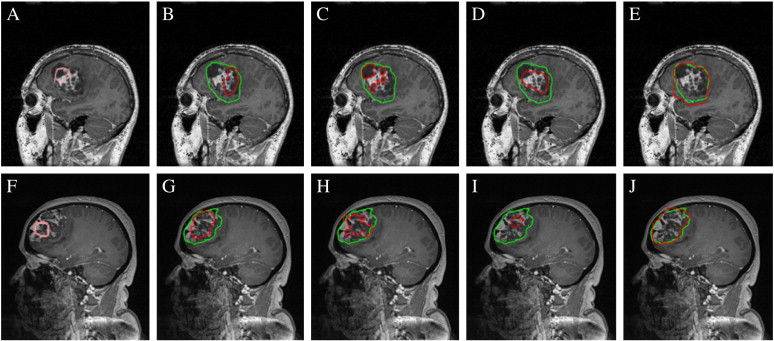
\includegraphics[width=1.7in, height=0.8in]{braintumor.jpg}
 \caption{Braintumours detected by means of image segmentation}
 \end{figure}
\myitem Face and fingerprint recognition.
\myitem Video surveillance.
\end{itemize}
\pause
\item Many different techniques.
\end{itemize}
\end{frame}

\begin{frame}
\frametitle{Algorithms from the scikit-image Python library}
\begin{itemize}
\item The Watershed\cite{scikit-image} algorithm.
\begin{figure}
 \centering
 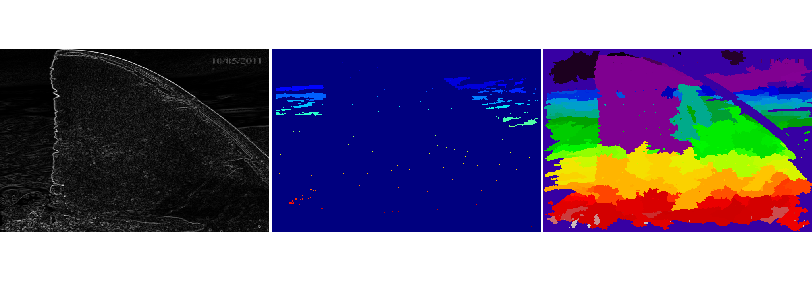
\includegraphics[width=1.7in, height=0.8in]{watershed.png}
 \caption{The Watershed algorithm}
 \end{figure}
\item The Random Walker\cite{scikit-image} algorithm.
\pause
\item The GrowCut algorithm performed exceptionally well.
\end{itemize}
\end{frame}

\begin{frame}
\frametitle{The region growing GrowCut segmentation algorithm}
\begin{itemize}
\item The GrowCut algorithm is an interactive, multi-label segmentation algorithm for N-dimensional images\cite{alg}.
\pause
\item How does it work? 
\begin{itemize}
\myitem Based on Cellular Automata\cite{cellularoutomata}.
\myitem Evolution rule/attacking strategy.
\myitem Neighbouring cells compared to the cell under consideration.  The state of this cell is then updated
according to the evolution rule.
\end{itemize}
\pause
\begin{figure}
\centering
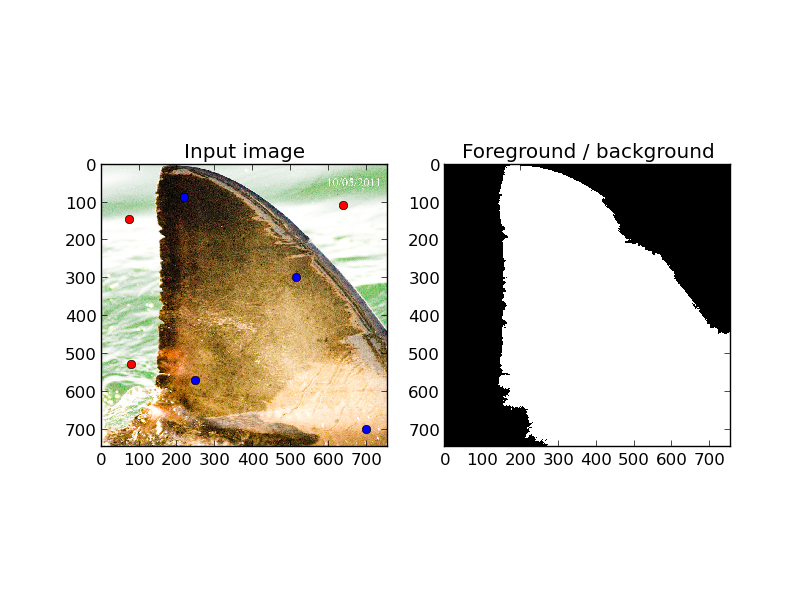
\includegraphics[width=2in, height=1in]{demo1.png}
\caption{The GrowCut algorithm}
\end{figure}
\end{itemize}
\end{frame}

\begin{frame}
\frametitle{The region growing GrowCut segmentation algorithm (cont)}
\begin{itemize}
\item Building a pipeline such that the input data is the shark fin image and the output is a specific
classification of that image.
\item Would want the orientation of all images to be the same.
\item Easier to specify foreground and background pixels.
\item Extract unique part of fin.
\end{itemize}
\end{frame}


\begin{frame}
\frametitle{DARWIN -- Alternative software}
\begin{itemize}
 \item An article appeared in Die Burger claiming that this
 software could also be used to estimate the size of the Great White shark
 population in the Gansbaai area by means of shark fin identification and
 matching.\cite{Darwin}
 \pause
 \item The validity of this claim was tested by Ms. Andreotti, which found it to
 be reliable in 54\% of the cases.
 \pause
 \item Produce more robust and reliable software.
\end{itemize}
\pause
\begin{figure}
 \centering
 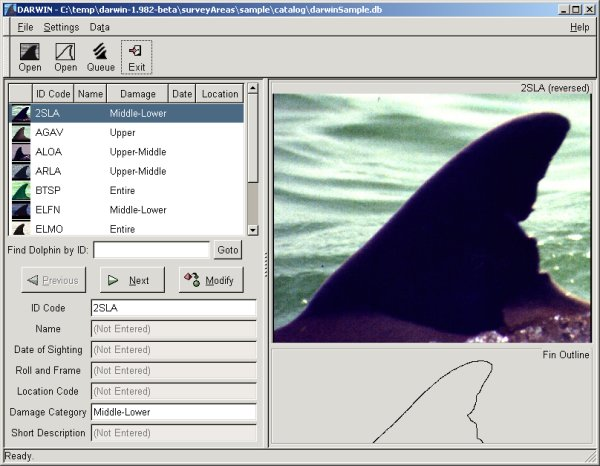
\includegraphics[width=1.5in, height=0.9in]{Darwin.jpg}
 \caption{User interface}
\end{figure}
\end{frame}


\begin{frame}
\frametitle{Concluding remarks}
\begin{itemize}
\item Future work
\begin{itemize}
 \myitem Pipeline and evolution rule.
\end{itemize}
\pause
\item Joy and satisfaction of a project of such applicability.
\pause
\item Thank project advisors for their guidance and support.
\end{itemize}
\end{frame}


\begin{frame}
\frametitle{Bibliography}
\bibliographystyle{plain}
\bibliography{ProjectProposalPresentation}
\end{frame}


\end{document}
